\chapter{Event- and LiDAR-Based Depth Estimation using a Convolutional Network}\label{sec:aled}

As noted in the conclusion of \cref{sec:ebof}, despite our good optical flow results, our experiments showed that their slight lack of precision was a critical issue if we wanted to exploit them further. In an objective to solve the ``depth'' part of the subject of the thesis, we started investigating the fusion of events with LiDAR data, in order to be able to estimate dense depth maps. Our approach also fundamentally changed: while the real-time, geometry-based approach for computing optical flow was an interesting problem to solve, we realized that it limited us in terms of accuracy, and that our results were starting to be difficult to defend compared to the most recent learning-based methods. The characteristics of the problem we aim to solve (detailed in \cref{sec:aled:two_depths_per_event}) also require a good understanding of the scene, which would be difficult to model with a purely geometry-based method. Therefore, we describe in this chapter an offline, learning-based approach for estimating dense depth maps from the fusion of LiDAR and event data.

The presented method and the associated results of this chapter were published as part of the 22nd Scandinavian Conference on Image Analysis in April 2023~\cite{Brebion2023LearningTE}. A project page is also available at \url{https://vbrebion.github.io/ALED/}, and contains the links to the original article, the source code, the dataset, and videos associated to this work.

\section{Introduction}\label{sec:aled:intro}
LiDAR sensors offer accurate but sparse 3D information of their surrounding environment. As noted in \cref{sec:intro}, they are a key component for intelligent robotic and autonomous navigation, helping to solve multiple problems, e.g., obstacle detection and tracking, SLAM, scene flow, etc. Yet, the sparsity of their point clouds often constitutes a limiting factor. While 64- or 128-channel LiDARs are starting to be commercialized, they come at a significantly high cost, and are still not as dense as cameras.

In this chapter, we focus on the fusion of LiDAR and event data, which we consider as a dual problem:
\begin{enumerate*}[label=\textbf{(\arabic*)}]
  \item LiDAR depths densification and\label{lst:aled:intro:densify}
  \item events-depths association.\label{lst:aled:intro:assign}
\end{enumerate*}
Regarding problem~\ref{lst:aled:intro:densify}, we are interested in densifying the LiDAR data using the events as a guide. As a result, dense depth maps are obtained, which allow for a dense 3D perception of the observed scene. As for problem~\ref{lst:aled:intro:assign}, we are interested in associating a depth to each event. By doing so, each event can be projected in 3D, and then even be backprojected in 2D in another vision sensor. For a fully calibrated and synced setup, this process would allow for the superimposition of events and RGB images from two different cameras for instance.

Estimating dense depth maps from sparse LiDAR data is a well-regarded problem as it solves the sparsity drawback of the LiDAR while keeping its metric scale. However, using events to densify depth maps (i.e., problem~\ref{lst:aled:intro:densify}) might inaccurately be seen as a task that inherently includes problem~\ref{lst:aled:intro:assign}, where corresponding depths for the events could be taken from the dense depth map. We argue in this chapter that, as each event represents a change in illumination, it might also represent a change in depth. As such, two depths should be associated to each event, and we will therefore compute two depth maps: one before the events happen, and one after they happen.

As an answer to these issues, we propose in this chapter a learning-based fusion method for estimating pairs of dense depth maps from events and sparse LiDAR data. For that purpose, we propose a novel convolutional network, the \acrfull{aled}, able to fuse asynchronous events and LiDAR data, and to estimate the two dense depth maps from them, while surpassing state-of-the-art accuracy. We also build a high-definition simulated dataset, the \acrfull{sled} dataset, used as part of the training of the network and its evaluation.

This chapter is structured as follows. We first give an overview of the state of the art in \cref{sec:aled:sota}. We then examine the duality of the problem and the issue of associating a single depth to each event in \cref{sec:aled:two_depths_per_event}. We give a detailed description of our \acrshort{aled} network and of our \acrshort{sled} dataset in \cref{sec:aled:method,sec:aled:sled} respectively. We finally conduct our evaluation in \cref{sec:aled:eval}, before drawing some conclusions in \cref{sec:aled:conclusion}.


\section{Related Work}\label{sec:aled:sota}

\subsection{LiDAR Densification}
Point clouds produced by LiDAR sensors are sparse, which is challenging for numerous applications (3D reconstruction, object detection, \acrshort{slam}, etc). As a consequence, LiDAR depth completion is a subject that has been widely studied in the literature.

Some authors try to obtain dense depth maps while only relying on the sparse data from the LiDAR. These methods either use machine learning~\cite{Uhrig2017SparsityIC,Chodosh2018DeepCC,Huang2020HMSNetHM} or traditional image processing operations~\cite{Ku2018InDO}.

The most successful approaches use a secondary modality as a guide for the densification process. While most of these approaches employ an RGB camera as the secondary sensor~\cite{Huang2020HMSNetHM,Jaritz2018SparseAD,VanGansbeke2019SparseAN,Xu2019DepthCF}, other authors have proposed using alternative modalities, such as stereo cameras~\cite{Maddern2016RealtimePF} or more recently event cameras~\cite{Cui2022DenseDE}.

\subsection{Fusion of Events and Other Modalities}
Due to their relative youth, the literature on the fusion of data from event cameras with other sensors is quite sparse.

Most of the investigations focused on the fusion of events and frames, thanks to sensors offering both modalities like the DAVIS camera~\cite{Brandli2014A2}. These works include frame interpolation and deblurring~\cite{Scheerlinck2018ContinuoustimeIE,Pan2019BringingAB,Paikin2021EFINetVF}, feature tracking~\cite{Kueng2016LowlatencyVO,Gehrig2019EKLTAP}, object detection~\cite{Jiang2019MixedFF,Cao2021FusionBasedFA,Tomy2022FusingEA}, or even steering prediction~\cite{Hu2020DDD20EE}.

In the past few years, a few authors have started investigating the fusion of events and LiDAR data. Explored issues concern primarily calibration~\cite{Song2018CalibrationOE,Ta2022L2ELT,Jiao2023LCECalibAL} and dataset construction~\cite{Zhu2018TheMS,Gehrig2021DSECAS,Chaney2023M3EDMM}. More recently, some works have been done on point clouds enhancement with events~\cite{Li2021Enhancing3L}, LiDAR densification~\cite{Cui2022DenseDE}, and human tracking in adversarial lighting conditions~\cite{Saucedo2023EventCA}.

\subsection{Depth Estimation with Events}
Several approaches have been proposed in order to estimate sparse or dense depth maps by using a single event camera. Kim \textit{et al.}~\cite{Kim2016RealTime3R} used probabilistic filters to simultaneously estimate the motion of the camera, reconstruct a log intensity image of the observed scene, and construct a sparse inverse depth map. Zhu \textit{et al.}~\cite{Zhu2019UnsupervisedEL} used a convolutional network to jointly predict depth and ego-motion, by trying to minimize the amount of motion blur in the accumulated events. Hidalgo-Carri\'o \textit{et al.}~\cite{HidalgoCarrio2020LearningMD} were the first to estimate dense depth maps, through the use of a recurrent convolutional network.

In parallel, other authors have advocated for the use of a secondary sensor to help the depth estimation. Schraml \textit{et al.}~\cite{Schraml2010DynamicSV,Schraml2016AnES} and Nam \textit{et al.}~\cite{Nam2022StereoDF} used two event cameras, and estimated depths by creating images of accumulated events for each camera and applying stereo matching. While~\cite{Schraml2010DynamicSV,Schraml2016AnES} used traditional model-based approaches, \cite{Nam2022StereoDF} entirely relied on learning-based networks: an attention-based network to construct detailed events representations, then a convolutional network for depth map inference. Other authors have also combined the event camera with an RGB sensor; Gehrig \textit{et al.}~\cite{Gehrig2021CombiningEA} for instance designed a recurrent network to fuse asynchronous data and estimate dense depths from them. Finally, some authors have also used depth sensors in direct combination with event cameras. Weikersdorfer \textit{et al.}~\cite{Weikersdorfer2014Eventbased3S} used an \mbox{RGB-D} camera to obtain dense depths, and used the depth-augmented events to perform \acrshort{slam}. Li \textit{et al.}~\cite{Li2021Enhancing3L} used a LiDAR sensor to associate a depth to each event through the use of a Voronoi diagram and a set of heuristic rules. Cui \textit{et al.}~\cite{Cui2022DenseDE} also employed a LiDAR, to derive dense depth maps by using 3D geometric information.


\section{Depth Change Map: Two Depths per Event}\label{sec:aled:two_depths_per_event}

In this chapter, we are interested in the fusion of LiDAR and event data. This problem is actually made of two complementary objectives:
\begin{enumerate*}[label=\textbf{(\arabic*)}]
  \item obtaining dense depth maps from events and sparse LiDAR data, and\label{lst:aled:dualpb:densify}
  \item assigning a depth to each event.\label{lst:aled:dualpb:assign}
\end{enumerate*}
While objective~\ref{lst:aled:dualpb:densify} can be interpreted as a LiDAR densification method guided by the events, we argue here for objective~\ref{lst:aled:dualpb:assign} that associating a single depth to an event is inadequate.

By definition, an event represents a significant change in illumination observed by a given pixel. Under motion, observed events can either originate from
\begin{enumerate*}[label=\textbf{(\alph*)}]
  \item texture changes inside an object; or from\label{lst:aled:evtsorigin:texture}
  \item the contour of an object.\label{lst:aled:evtsorigin:contour}
\end{enumerate*}
In case~\ref{lst:aled:evtsorigin:texture}, associating a single depth to these events can be coherent, as depth inside an object should be subject to little variation. However, doing so in case~\ref{lst:aled:evtsorigin:contour} is erroneous, as events happening at contours of objects are likely to denote also a depth change. This reflection is analogous to the one described in the conclusion of the chapter on optical flow (\cref{sec:ebof:conclusion}): we want here to take into account the ``change-based'' nature of events, and not reproduce the common error of merely considering them as a snapshot of the texture and edges of the objects in the scene.

\begin{figure}
  \centering
  \begin{subfigure}{0.475\linewidth}
    \centering
    \includegraphics[width=\textwidth]{mainmatter/figures/4_depth_conv/depth_diff_example/gtprev000015.png}
    \caption{Ground truth for \(D_\text{bf}\)}
  \end{subfigure}
  \begin{subfigure}{0.475\linewidth}
    \centering
    \includegraphics[width=\textwidth]{mainmatter/figures/4_depth_conv/depth_diff_example/gtcurr000015.png}
    \caption{Ground truth for \(D_\text{af}\)}
  \end{subfigure}
  \begin{subfigure}{\linewidth}
    \centering
    \raisebox{-0.5\height}{\includegraphics[width=0.5\textwidth]{mainmatter/figures/4_depth_conv/depth_diff_example/gtdiff000015.png}}
    \raisebox{-0.5\height}{
      \begin{tikzpicture}
        \definecolor{colorblack}{HTML}{000004}
        \definecolor{coloryellow}{HTML}{FCFFA4}
        \definecolor{colorpink}{HTML}{BC3754}
        \node[] (title) {Thresholds:};
        \node[draw, minimum width=0.25cm, minimum height=0.25cm, fill=colorblack, below left=0.5cm and -0.4cm of title] (black) {};
        \node[draw, minimum width=0.25cm, minimum height=0.25cm, fill=colorpink, below=0.5cm of black] (pink) {};
        \node[draw, minimum width=0.25cm, minimum height=0.25cm, fill=coloryellow, below=0.5cm of pink] (yellow) {};
        \node[right=0.1cm of black] (black_l) {\(d_\text{af} - d_\text{bf} < -1\text{m}\)};
        \node[right=0.1cm of pink] (pink_l) {\(d_\text{af} - d_\text{bf} \in [-1\text{m}, +1\text{m}]\)};
        \node[right=0.1cm of yellow] (yellow_l) {\(d_\text{af} - d_\text{bf} > +1\text{m}\)};
      \end{tikzpicture}
    }
    \caption{Thresholded depth change map, using the events as a mask}
  \end{subfigure}
  \cprotect\caption{Example of the importance of the depth change map for each event on the \verb|Town01_00| sequence from our \acrshort{sled} dataset. Notice how simple thresholds on this depth difference help distinguishing the events linked to the contour of real objects from the events corresponding to the texture of the road, the halo from the streetlamp, or even the noisy events in the sky.}\label{fig:aled:depth_difference_example}
\end{figure}

Therefore, we propose here to always associate \textit{two} depths to each event to take into account this potential change of depth: the depth of the pixel \textit{before} the event (the change) occurred, and the depth of the pixel \textit{after} the event occurred. Associating directly a single ``depth change'' value to each event could be viewed as an alternative, but we argue that absolute depth values are much more important, as they are required in numerous applications. As we are interested in solving both objective \ref{lst:aled:dualpb:densify} and \ref{lst:aled:dualpb:assign} simultaneously, we estimate here two dense depth maps: one before the events occur, which we will denote \(D_\text{bf}\) in the rest of this chapter, and one after the events occur, which we will denote \(D_\text{af}\). We can then formulate the depth change map as \(\Delta D \doteq D_\text{af}-D_\text{bf}\) and compare the depth change \(\Delta d \doteq d_\text{af}-d_\text{bf}\) for each pixel. Three meaningful cases can be distinguished:
\begin{enumerate}
  \item \(\Delta d \approx 0\): the pixel is located in an area where depths do not vary much, i.e., inside an object;
  \item \(\Delta d \gg 0\): the pixel was at the edge of an object, and is now on an object further away;
  \item \(\Delta d \ll 0\): the pixel was located on a far object, and is now at the edge of a closer object.
\end{enumerate}

The depth difference information given by the depth change map can especially help to process events to differentiate real object edges from textures or artifacts such as shadows and even noise. An illustration of some possibilities offered by the depth change map on events is given in \cref{fig:aled:depth_difference_example}. Other applications could also take advantage of the pair of depth maps \(D_\text{bf}\) and \(D_\text{af}\): ego-motion and speed estimation, objects clustering, scene flow, etc.


\section{Method}\label{sec:aled:method}

\subsection{The ALED Network}

\begin{figure}
  \centering
  \resizebox{0.85\textwidth}{!}{
    \begin{tikzpicture}[every node/.style={inner sep=0.001,outer sep=0.001}]
      % Defining the colors that will be used for the network
      \definecolor{color_l}{RGB}{204,187,68}
      \definecolor{color_e}{RGB}{238,102,119}
      \definecolor{color_le}{RGB}{68,119,170}
      \definecolor{color_ee}{RGB}{68,119,170}
      \definecolor{color_gru}{RGB}{187,187,187}

      % Changing the font
      \fontfamily{cmss}\selectfont

      % LiDAR encoders
      \node[] (L) at (0,0) {\includegraphics[width=0.2\textwidth,cfbox=color_l 0.05cm 0pt]{mainmatter/figures/4_depth_conv/network/lidar_lightgray_fixed.png}};
      \node[above=0.1cm of L] (Ll) {LiDAR};

      \node[draw, trapezium, minimum width=1cm, right=1.5cm of L, opacity=0.0] (tmplh) {};
      \node[draw, trapezium, minimum width=1cm, fill=color_l, rotate around={-90:(tmplh.center)}] (LH) at (tmplh) {};

      \node[draw, trapezium, minimum width=1cm, on grid, right=2.5cm of tmplh, opacity=0.0] (tmple1) {};
      \node[draw, trapezium, minimum width=1cm, fill=color_le, rotate around={-90:(tmple1.center)}] (LE1) at (tmple1) {};

      \node[draw, trapezium, minimum width=1cm, on grid, right=2.5cm of tmple1, opacity=0.0] (tmple2) {};
      \node[draw, trapezium, minimum width=1cm, fill=color_le, rotate around={-90:(tmple2.center)}] (LE2) at (tmple2) {};

      \node[draw, trapezium, minimum width=1cm, on grid, right=2.5cm of tmple2, opacity=0.0] (tmple3) {};
      \node[draw, trapezium, minimum width=1cm, fill=color_le, rotate around={-90:(tmple3.center)}] (LE3) at (tmple3) {};

      \draw[->,>=latex, line width=0.5mm, color_l] (L) -- node [above=0.1cm, midway] (al1) {1} (LH);
      \draw[->,>=latex, line width=0.5mm, color_l] (LH) -- node [above=0.1cm, midway] (al2) {32} (LE1);
      \draw[->,>=latex, line width=0.5mm, color_l] (LE1) -- node [above=0.1cm, midway] (al3) {64} (LE2);
      \draw[->,>=latex, line width=0.5mm, color_l] (LE2) -- node [above=0.1cm, midway] (al4) {128} (LE3);

      % ConvGRUs
      \node[draw, minimum width=0.75cm, minimum height=0.75cm, fill=color_gru, on grid, below right=1.5cm and 1.25cm of tmplh] (CGRUL1) {};
      \node[draw, minimum width=0.75cm, minimum height=0.75cm, fill=color_gru, on grid, below right=1.5cm and 1.25cm of tmple1] (CGRUL2) {};
      \node[draw, minimum width=0.75cm, minimum height=0.75cm, fill=color_gru, on grid, below right=1.5cm and 1.25cm of tmple2] (CGRUL3) {};
      \node[draw, minimum width=0.75cm, minimum height=0.75cm, fill=color_gru, on grid, below right=1.5cm and 1.25cm of tmple3] (CGRUL4) {};

      % LiDAR -> ConvGRUs
      \draw[->,>=latex, line width=0.5mm, color_l] (LH -| al2) -- (CGRUL1);
      \draw[->,>=latex, line width=0.5mm, color_l] (LE1 -| al3) -- (CGRUL2);
      \draw[->,>=latex, line width=0.5mm, color_l] (LE2 -| al4) -- (CGRUL3);
      \draw[->,>=latex, line width=0.5mm, color_l] (LE3) -| node [above=0.1cm, midway] {256} (CGRUL4);

      % Events encoders
      \node[on grid, below=7cm of L] (E) {\includegraphics[width=0.2\textwidth,cfbox=color_e 0.05cm 0pt]{mainmatter/figures/4_depth_conv/network/evts_lightgray_fixed.png}};
      \node[above=0.1cm of E] (El) {Events};

      \node[draw, trapezium, minimum width=1cm, right=1.5cm of E, opacity=0.0] (tmpeh) {};
      \node[draw, trapezium, minimum width=1cm, fill=color_e, rotate around={-90:(tmpeh.center)}] (EH) at (tmpeh) {};

      \node[draw, trapezium, minimum width=1cm, on grid, right=2.5cm of tmpeh, opacity=0.0] (tmpee1) {};
      \node[draw, trapezium, minimum width=1cm, fill=color_ee, rotate around={-90:(tmpee1.center)}] (EE1) at (tmpee1) {};

      \node[draw, trapezium, minimum width=1cm, on grid, right=2.5cm of tmpee1, opacity=0.0] (tmpee2) {};
      \node[draw, trapezium, minimum width=1cm, fill=color_ee, rotate around={-90:(tmpee2.center)}] (EE2) at (tmpee2) {};

      \node[draw, trapezium, minimum width=1cm, on grid, right=2.5cm of tmpee2, opacity=0.0] (tmpee3) {};
      \node[draw, trapezium, minimum width=1cm, fill=color_ee, rotate around={-90:(tmpee3.center)}] (EE3) at (tmpee3) {};

      \draw[->,>=latex, line width=0.5mm, color_e] (E) -- node [below=0.1cm, midway] (ae1) {10} (EH);
      \draw[->,>=latex, line width=0.5mm, color_e] (EH) -- node [below=0.1cm, midway] (ae2) {32} (EE1);
      \draw[->,>=latex, line width=0.5mm, color_e] (EE1) -- node [below=0.1cm, midway] (ae3) {64} (EE2);
      \draw[->,>=latex, line width=0.5mm, color_e] (EE2) -- node [below=0.1cm, midway] (ae4) {128} (EE3);

      % ConvGRUs
      \node[draw, minimum width=0.75cm, minimum height=0.75cm, on grid, fill=color_gru, above right=1.5cm and 1.25cm of tmpeh] (CGRUE1) {};
      \node[draw, minimum width=0.75cm, minimum height=0.75cm, on grid, fill=color_gru, above right=1.5cm and 1.25cm of tmpee1] (CGRUE2) {};
      \node[draw, minimum width=0.75cm, minimum height=0.75cm, on grid, fill=color_gru, above right=1.5cm and 1.25cm of tmpee2] (CGRUE3) {};
      \node[draw, minimum width=0.75cm, minimum height=0.75cm, on grid, fill=color_gru, above right=1.5cm and 1.25cm of tmpee3] (CGRUE4) {};

      % Events -> convGRUs
      \draw[->,>=latex, line width=0.5mm, color_e] (EH -| ae2) -- (CGRUE1);
      \draw[->,>=latex, line width=0.5mm, color_e] (EE1 -| ae3) -- (CGRUE2);
      \draw[->,>=latex, line width=0.5mm, color_e] (EE2 -| ae4) -- (CGRUE3);
      \draw[->,>=latex, line width=0.5mm, color_e] (EE3) -| node [below=0.1cm, midway] {256} (CGRUE4);

      % ConvGRUs states
      \node[draw, minimum width=1cm, minimum height=1cm, on grid, below=2cm of CGRUL1] (S1) {1/1};
      \node[draw, minimum width=1cm, minimum height=1cm, on grid, below=2cm of CGRUL2] (S2) {1/2};
      \node[draw, minimum width=1cm, minimum height=1cm, on grid, below=2cm of CGRUL3] (S3) {1/4};
      \node[draw, minimum width=1cm, minimum height=1cm, on grid, below=2cm of CGRUL4] (S4) {1/8};

      % LiDAR convGRUs <-> convGRU states
      \draw[->,>=latex, line width=0.5mm, color_l] (CGRUL1) -- node [right=0.15cm, midway, align=left] {\textcolor{red}{32}\textcolor{black}{+}\\\textcolor{Purple}{32}} (S1);
      \draw[line width=0.5mm, color_gru] (S1.west) -- ($(S1.west)+(-0.25cm,0)$);
      \draw[->,>=latex, line width=0.5mm, color_gru] ($(S1.west)+(-0.25cm,0)$) |- (CGRUL1.west);
      \draw[->,>=latex, line width=0.5mm, color_l] (CGRUL2) -- node [right=0.15cm, midway, align=left] {\textcolor{red}{64}\textcolor{black}{+}\\\textcolor{Purple}{64}} (S2);
      \draw[line width=0.5mm, color_gru] (S2.west) -- ($(S2.west)+(-0.25cm,0)$);
      \draw[->,>=latex, line width=0.5mm, color_gru] ($(S2.west)+(-0.25cm,0)$) |- (CGRUL2.west);
      \draw[->,>=latex, line width=0.5mm, color_l] (CGRUL3) -- node [right=0.15cm, midway, align=left] {\textcolor{red}{128}\textcolor{black}{+}\\\textcolor{Purple}{128}} (S3);
      \draw[line width=0.5mm, color_gru] (S3.west) -- ($(S3.west)+(-0.25cm,0)$);
      \draw[->,>=latex, line width=0.5mm, color_gru] ($(S3.west)+(-0.25cm,0)$) |- (CGRUL3.west);
      \draw[->,>=latex, line width=0.5mm, color_l] (CGRUL4) -- node [right=0.15cm, midway, align=left] {\textcolor{red}{256}} (S4);
      \draw[line width=0.5mm, color_gru] (S4.west) -- ($(S4.west)+(-0.25cm,0)$);
      \draw[->,>=latex, line width=0.5mm, color_gru] ($(S4.west)+(-0.25cm,0)$) |- (CGRUL4.west);

      % Events convGRUs <-> convGRU states
      \draw[->,>=latex, line width=0.5mm, color_e] (CGRUE1) -- node [right=0.15cm, midway, align=left] {\textcolor{red}{32}\textcolor{black}{+}\\\textcolor{Purple}{32}} (S1);
      \draw[->,>=latex, line width=0.5mm, color_gru] ($(S1.west)+(-0.25cm,0)$) |- (CGRUE1.west);
      \draw[->,>=latex, line width=0.5mm, color_e] (CGRUE2) -- node [right=0.15cm, midway, align=left] {\textcolor{red}{64}\textcolor{black}{+}\\\textcolor{Purple}{64}} (S2);
      \draw[->,>=latex, line width=0.5mm, color_gru] ($(S2.west)+(-0.25cm,0)$) |- (CGRUE2.west);
      \draw[->,>=latex, line width=0.5mm, color_e] (CGRUE3) -- node [right=0.15cm, midway, align=left] {\textcolor{red}{128}\textcolor{black}{+}\\\textcolor{Purple}{128}} (S3);
      \draw[->,>=latex, line width=0.5mm, color_gru] ($(S3.west)+(-0.25cm,0)$) |- (CGRUE3.west);
      \draw[->,>=latex, line width=0.5mm, color_e] (CGRUE4) -- node [right=0.15cm, midway, align=left] {\textcolor{red}{256}} (S4);
      \draw[->,>=latex, line width=0.5mm, color_gru] ($(S4.west)+(-0.25cm,0)$) |- (CGRUE4.west);

      % Legend
      \node[draw, trapezium, minimum width=1cm, below right=1.5cm and -1.5cm of E, opacity=0.0] (tmpllh) {};
      \node[draw, trapezium, minimum width=1cm, fill=color_l, rotate around={-90:(tmpllh.center)}] (LLH) at (tmpllh) {};
      \node[right=0.1cm of tmpllh] (LLHT) {LiDAR head};

      \node[draw, trapezium, minimum width=1cm, below= of tmpllh, opacity=0.0] (tmpleh) {};
      \node[draw, trapezium, minimum width=1cm, fill=color_e, rotate around={-90:(tmpleh.center)}] (LEH) at (tmpleh) {};
      \node[right=0.1cm of tmpleh] (LEHT) {Events head};

      \node[draw, trapezium, minimum width=1cm, below right=0.4cm and 1cm of LLHT, opacity=0.0] (tmpllee) {};
      \node[draw, trapezium, minimum width=1cm, fill=color_le, rotate around={-90:(tmpllee.center)}] (LLEE) at (tmpllee) {};
      \node[right=0.1cm of tmpllee, align=left] (LLEET) {LiDAR/Events\\encoder};

      \node[draw, minimum width=0.75cm, minimum height=0.75cm, fill=color_gru, right=5cm of LLHT] (LCGRU) {};
      \node[right=0.325cm of LCGRU] (LCGRUT) {convGRU};

      \node[draw, minimum width=1cm, minimum height=1cm] at (LEHT -| LCGRU) (LS) {\(S\)};
      \node[right=0.2cm of LS, align=left] (LST) {convGRU state\\(scale \(S\))};
    \end{tikzpicture}
  }
  \caption{The encoder part of the network. The numbers along the connections indicate the number of channels of the corresponding data.}\label{fig:aled:encoder}

  \vspace{20mm}

  \resizebox{\textwidth}{!}{
    \begin{tikzpicture}[every node/.style={inner sep=0.001,outer sep=0.001}]
      % Defining the colors that will be used for the network
      \definecolor{color_d}{RGB}{34,136,51}
      \definecolor{color_cu}{RGB}{170,51,119}
      \definecolor{color_c}{RGB}{102,204,238}
      \definecolor{color_res}{RGB}{187,187,187}

      % Changing the font
      \fontfamily{cmss}\selectfont

      % First convGRU state and residual blocks
      \node[draw, minimum width=1cm, minimum height=1cm] (S4) {1/8};
      \node[draw, minimum width=0.75cm, minimum height=0.75cm, fill=color_res, on grid, below=2cm of S4] (Res1) {};
      \node[draw, minimum width=0.75cm, minimum height=0.75cm, fill=color_res, right=0.75cm of Res1] (Res2) {};

      % Upsampling guided by second convGRU state, concat and conv
      \node[draw, trapezium, minimum width=1cm, right=0.75cm of Res2, opacity=0.0] (tmpu1) {};
      \node[draw, trapezium, minimum width=1cm, fill=color_cu, rotate around={90:(tmpu1.center)}] (U1) at (tmpu1) {};
      \node[draw, circle, minimum width=0.5cm, right=0.75cm of tmpu1] (C1) {C};
      \node[draw, minimum width=1cm, minimum height=1cm, on grid, above=2cm of C1] (S3) {1/4};
      \node[draw, trapezium, minimum width=1cm, right=0.75cm of C1, opacity=0.0] (tmpconv1) {};
      \node[draw, trapezium, minimum width=1cm, fill=color_c, rotate around={-90:(tmpconv1.center)}] (conv1) at (tmpconv1) {};

      % Upsampling guided by third convGRU state, concat and conv
      \node[draw, trapezium, minimum width=1cm, right=0.75cm of tmpconv1, opacity=0.0] (tmpu2) {};
      \node[draw, trapezium, minimum width=1cm, fill=color_cu, rotate around={90:(tmpu2.center)}] (U2) at (tmpu2) {};
      \node[draw, circle, minimum width=0.5cm, right=0.5cm of tmpu2] (C2) {C};
      \node[draw, minimum width=1cm, minimum height=1cm, on grid, above=2cm of C2] (S2) {1/2};
      \node[draw, trapezium, minimum width=1cm, right=0.75cm of C2, opacity=0.0] (tmpconv2) {};
      \node[draw, trapezium, minimum width=1cm, fill=color_c, rotate around={-90:(tmpconv2.center)}] (conv2) at (tmpconv2) {};

      % Upsampling guided by fourth convGRU state, concat and conv
      \node[draw, trapezium, minimum width=1cm, right=0.5cm of tmpconv2, opacity=0.0] (tmpu3) {};
      \node[draw, trapezium, minimum width=1cm, fill=color_cu, rotate around={90:(tmpu3.center)}] (U3) at (tmpu3) {};
      \node[draw, circle, minimum width=0.5cm, right=0.5cm of tmpu3] (C3) {C};
      \node[draw, minimum width=1cm, minimum height=1cm, on grid, above=2cm of C3] (S1) {1/1};
      \node[draw, trapezium, minimum width=1cm, right=0.5cm of C3, opacity=0.0] (tmpconv3) {};
      \node[draw, trapezium, minimum width=1cm, fill=color_c, rotate around={-90:(tmpconv3.center)}] (conv3) at (tmpconv3) {};

      % Prediction head
      \node[draw, trapezium, minimum width=1cm, right=0.5cm of tmpconv3, opacity=0.0] (tmpp) {};
      \node[draw, trapezium, minimum width=1cm, fill=color_d, rotate around={-90:(tmpp.center)}] (P) at (tmpp) {};
      \node[right=0.5cm of tmpp] (out) {
        \begin{tikzpicture}
          \node[on grid] (Daf) {\includegraphics[width=0.185\textwidth,cfbox=color_d 0.05cm 0pt]{mainmatter/figures/4_depth_conv/network/prev.png}};
          \node[on grid, below left=0.25cm and 0.25cm of Daf] (Dbf) {\includegraphics[width=0.185\textwidth,cfbox=color_d 0.05cm 0pt]{mainmatter/figures/4_depth_conv/network/prev.png}};
        \end{tikzpicture}
      };
      \node[above=0.1cm of out, align=center] (outl) {Dense depths\\\(D_\text{bf}\) and \(D_\text{af}\)};

      % Paths
      \draw[->,>=latex, line width=0.5mm, color_res] (S4) -- node [right=0.15cm, midway, align=center] {\textcolor{red}{256}} (Res1);
      \draw[->,>=latex, line width=0.5mm, color_d] (Res1) -- node [below=0.15cm, midway, align=center] {256} (Res2);
      \draw[->,>=latex, line width=0.5mm, color_d] (Res2) -- node [below=0.15cm, midway, align=center] {256} (U1);
      \draw[->,>=latex, line width=0.5mm, color_res] (S3) -| node [above=0.15cm, midway, align=center] {\textcolor{Purple}{128}} (U1);
      \draw[->,>=latex, line width=0.5mm, color_res] (S3) -- node [right=0.15cm, midway, align=center] {\textcolor{red}{128}} (C1);
      \draw[->,>=latex, line width=0.5mm, color_d] (U1) -- node [below=0.15cm, midway, align=center] {128} (C1);
      \draw[->,>=latex, line width=0.5mm, color_d] (C1) -- node [below=0.15cm, midway, align=center] {256} (conv1);
      \draw[->,>=latex, line width=0.5mm, color_d] (conv1) -- node [below=0.15cm, midway, align=center] {128} (U2);
      \draw[->,>=latex, line width=0.5mm, color_res] (S2) -| node [above=0.15cm, midway, align=center] {\textcolor{Purple}{64}} (U2);
      \draw[->,>=latex, line width=0.5mm, color_res] (S2) -- node [right=0.15cm, midway, align=center] {\textcolor{red}{64}} (C2);
      \draw[->,>=latex, line width=0.5mm, color_d] (U2) -- node [below=0.15cm, midway, align=center] {64} (C2);
      \draw[->,>=latex, line width=0.5mm, color_d] (C2) -- node [below=0.15cm, midway, align=center] {128} (conv2);
      \draw[->,>=latex, line width=0.5mm, color_d] (conv2) -- node [below=0.15cm, midway, align=center] {64} (U3);
      \draw[->,>=latex, line width=0.5mm, color_res] (S1) -| node [above=0.15cm, midway, align=center] {\textcolor{Purple}{32}} (U3);
      \draw[->,>=latex, line width=0.5mm, color_res] (S1) -- node [right=0.15cm, midway, align=center] {\textcolor{red}{32}} (C3);
      \draw[->,>=latex, line width=0.5mm, color_d] (U3) -- node [below=0.15cm, midway, align=center] {32} (C3);
      \draw[->,>=latex, line width=0.5mm, color_d] (C3) -- node [below=0.15cm, midway, align=center] {64} (conv3);
      \draw[->,>=latex, line width=0.5mm, color_d] (conv3) -- node [below=0.15cm, midway, align=center] {32} (P);
      \draw[->,>=latex, line width=0.5mm, color_d] (P) -- node [below=0.15cm, midway, align=center] {2} (out);

      % Legend
      \node[draw, minimum width=1cm, minimum height=1cm, below right=1.5cm and 2.5cm of Res1] (LS) {\(S\)};
      \node[right=0.2cm of LS, align=left] (LST) {convGRU state\\(scale \(S\))};

      \node[draw, minimum width=0.75cm, minimum height=0.75cm, fill=color_res, right= of LST] (LRes) {};
      \node[right=0.2cm of LRes] (LResT) {Residual block};

      \node[draw, trapezium, minimum width=1cm, right=0.5cm of LResT, opacity=0.0] (tmplu) {};
      \node[draw, trapezium, minimum width=1cm, fill=color_cu, rotate around={90:(tmplu.center)}] (LU) at (tmplu) {};
      \node[right=0.1cm of tmplu] (LUT) {Convex upsampling};

      \node[draw, circle, minimum width=0.5cm, below=0.5cm of LS] (LC) {C};
      \node[right=0.45cm of LC] (LCT) {Concatenation};

      \node[draw, trapezium, minimum width=1cm, opacity=0.0] at (LC -| LRes) (tmplconv) {};
      \node[draw, trapezium, minimum width=1cm, fill=color_c, rotate around={-90:(tmplconv.center)}] (Lconv) at (tmplconv) {};
      \node[right=0.2cm of tmplconv] (LconvT) {Convolution};

      \node[draw, trapezium, minimum width=1cm, opacity=0.0] at (tmplconv -| tmplu) (tmplpred) {};
      \node[draw, trapezium, minimum width=1cm, fill=color_d, rotate around={-90:(tmplpred.center)}] (Lpred) at (tmplpred) {};
      \node[right=0.1cm of tmplpred] (LpredT) {Prediction head};
    \end{tikzpicture}
  }
  \caption{The decoder part of the network. The numbers along the connections indicate the number of channels of the corresponding data.}\label{fig:aled:decoder}
\end{figure}

Inspired by the Recurrent Asynchronous Multimodal Network (RAMNet) architecture of Gehrig \textit{et al.}~\cite{Gehrig2021CombiningEA} for RGB and events fusion, we propose here a fully convolutional recurrent network to estimate dense depth maps from asynchronous LiDAR and events data. We call it \acrshort{aled}, for \acrlong{aled}.

\acrshort{aled} can be decomposed in two main parts: an encoder, tasked with fusing asynchronous events and LiDAR features at different scales, and a decoder, tasked with interpreting the fused features for estimating dense depths. Both of them are illustrated in \cref{fig:aled:encoder,fig:aled:decoder}.

\paragraph{Data Encoding}
In the encoder part, illustrated in \cref{fig:aled:encoder}, the LiDAR and events inputs are fed independently. Both of them go through an encoding head, computing a first feature map of 32 channels while keeping their original height and width. Convolutional encoders (in the form of ResNet Basic Blocks~\cite{He2016DeepRL}) are then used to compute feature maps at scales \(1/2\), \(1/4\), and \(1/8\), doubling the number of channels every time.

\paragraph{States Update}
Each feature map is used as the input of convolutional Gated Recurrent Unit (convGRU) blocks~\cite{Siam2017ConvolutionalGR}, updating the state at its corresponding scale. These states share a double purpose:
\begin{enumerate*}[label=\textbf{(\arabic*)}]
  \item they act as memories, making the network able to produce correct depth maps even in the case where the event camera would become static and thus not produce any event anymore, and
  \item since they are shared between the LiDAR and events encoders, both parts of the network can update them independently, allowing for an asynchronous fusion of the two modalities.
\end{enumerate*}

\paragraph{Decoding}
In its decoder part, illustrated in \cref{fig:aled:decoder}, the convGRU state at the lowest scale first goes through two residual blocks. Then, for each following scale, the decoded feature map from the previous scale is upscaled by using convex upsampling~\cite{Teed2020RAFTRA}. While a simple bilinear upsampling was used in RAMNet~\cite{Gehrig2021CombiningEA}, convex upsampling allows our network to learn how to upscale features from a lower scale, using information from a higher scale. We propose to design the convGRU such that the first half of its state (in purple in \cref{fig:aled:encoder,fig:aled:decoder}) guides the convex upsampling. Fusion of the upsampled decoded features and the state from the current scale is then performed by concatenating the output of the convex upsampling block with the remaining half of the convGRU state (in green in \cref{fig:aled:encoder,fig:aled:decoder}), and by applying a convolution to reduce the number of channels. After the last scale, a prediction head is used to obtain the two final depth maps, \(D_\text{bf}\) and \(D_\text{af}\), in the form of a two-channel tensor, at the same full resolution as the events input.

\subsection{Implementation}
Regarding the implementation of \acrshort{aled}, both encoding heads use a kernel size of 5. LiDAR and events encoders use a kernel size of 5, with stride 2. Both the convGRU and residual blocks use a kernel size of 3. The convolutions in the convex upsampling blocks use a kernel size of 5, while the convolutions following the concatenations use a kernel size of 1. Finally, the prediction layer also uses a kernel size of 1. Convolutions are followed by a PReLU activation function~\cite{He2015DelvingDI}, and instance normalization is used in the ResNet encoders as proposed by Pan \textit{et al.}~\cite{Pan2018TwoAO}. In total, the network contains 26 million trainable parameters.

\subsection{Data Representation}

\paragraph{Events}
We use the Event Volume~\cite{Zhu2019UnsupervisedEL} as the input representation for the events. We follow here the formulation of Perot \textit{et al.}~\cite{Perot2020LearningTD}, where, for input events \(\{e_i = (\mathbf{x}_i, p_i, t_i)\}_{i=1}^N\), the content of the Event Volume \(V\) for the pixel \(\mathbf{x}\), the polarity \(p\), and the bin \(b\) is defined as:
\begin{equation}
V(\mathbf{x}, p, b) \doteq \sum_{\{e_i | \mathbf{x}_i=\mathbf{x}, p_i=p\}} \max(0, 1-|b-t_i^*|),
\end{equation}
where \(t_i^*\) is defined as:
\begin{equation}
t_i^* \doteq (B-1)\frac{t_i-t_1}{t_N-t_1}
\end{equation}
and where \(B\) is the number of temporal bins to split the timestamps of the events.

In our experiments, we set \(B=5\text{ bins}\), and concatenate the negative and positive polarity bins along the first dimension, resulting in a 3D tensor of shape \((10, H, W)\).

\paragraph{LiDAR and Depths}
LiDAR data is fed to the network as a 1-channel depth image. To do so, each LiDAR point cloud is projected onto the image plane of the event camera. Pixels where one or more LiDAR points fall into are given as value the lowest depth. Pixels without any LiDAR point are given a value of 0. For an easier learning, the LiDAR projection and ground truth images are normalized between 0 and 1 based on the maximum LiDAR range (200m in the case of our synthetic \acrshort{sled} dataset, 100m in the case of the MVSEC dataset~\cite{Zhu2018TheMS}).

\subsection{Loss Functions}\label{sec:aled:method:loss}
To train our network, we combine the use of two losses: a pixel-wise \(\ell_1\) loss \(\mathcal{L}_\text{pw}\), and a multiscale gradient matching loss \(\mathcal{L}_\text{msg}\).

The pixel-wise \(\ell_1\) loss operates as the main supervision loss, applied on both the ``before'' and the ``after'' depth maps, and is defined as follows:
\begin{equation}
  \mathcal{L}_\text{pw} = \sum_{\mathbf{x}} \left\lVert D(\mathbf{x}) - \hat{D}(\mathbf{x}) \right\rVert _1
\end{equation}
where \(D\) and \(\hat{D}\) are respectively the estimated and ground truth depth maps. 

However, when supervised by the \(\ell_1\) loss alone, the network tends to produce blurry and non-smooth depth images. To solve this issue, we use here a multiscale gradient matching loss inspired by~\cite{Ummenhofer2017DeMoNDA}, also applied on both the ``before'' and the ``after'' depth maps, and defined as
\begin{equation}
  \mathcal{L}_\text{msg} = \sum_{h \in \{1, 2, 4, 8, 16\}} \sum_{\mathbf{x}} \left\lVert \text{\textbf{g}}[D](\mathbf{x}, h) - \text{\textbf{g}}[\hat{D}](\mathbf{x}, h) \right\rVert _2
\end{equation}
with the discrete gradient function \textbf{g} of an image \(f\) defined as
\begin{equation}
  \text{\textbf{g}}[f](x, y, h) = \begin{pmatrix} f(x+h, y) - f(x, y)\\ f(x, y+h) - f(x, y) \end{pmatrix}
\end{equation}
This loss helps to regulate the depth results, by making depth discontinuities more prominent, and by smoothing homogeneous regions.

Our total loss \(\mathcal{L}\) for a sequence of length \(T\) is finally defined as
\begin{equation}
  \mathcal{L} = \sum_{t=1}^T \sum_{\text{bf}, \text{af}} (\mathcal{L}_{\text{pw}}^t + \alpha \mathcal{L}_{\text{msg}}^t)
\end{equation}
where \(\alpha\) is a weight parameter for the multiscale gradient matching loss.

In our experiments, we observed that giving too much importance to the multiscale gradient matching loss early in the training makes the network unable to derive correct depth estimates. Therefore, we always set \(\alpha = 0.1\) during the first epoch of training, to force the network to use mainly the \(\ell_1\) loss and converge towards good initial depth estimates. For the remaining epochs, we set \(\alpha = 1\).


\section{The SLED Dataset}\label{sec:aled:sled}
In order to train and evaluate the proposed \acrshort{aled} network, we require a dataset containing both events, LiDAR point clouds, and a dense ground truth on depths. While we can use the MVSEC dataset~\cite{Zhu2018TheMS} for low-resolution cameras, its ground truth is constructed by accumulating point clouds from a LiDAR sensor, a solution which introduces errors in case of moving objects, as noted in \cref{sec:evtcams:datasets:mvsec}. In high-resolution, the DSEC dataset~\cite{Gehrig2021DSECAS} would have been a perfect candidate, but its ground truth depth maps are given at the timestamps of the RGB frames and not those of the LiDAR point clouds\footnote{For more details, see the following comment made by the authors of the DSEC dataset: \url{https://github.com/uzh-rpg/DSEC/issues/7\#issuecomment-1416776152}}, making these depth maps incompatible with the training and evaluation procedures of our network.

For these reasons, we use the CARLA simulator~\cite{Dosovitskiy2017CARLAAO} (version 0.9.14) to generate a dataset with perfect synchronization and calibration of the sensors, and perfect ground truth depth. We call it \acrshort{sled}, for \acrlong{sled} dataset. It is composed of 160 sequences of 10 seconds each, for a total of more than 20 minutes of data. These sequences are recorded on the \verb|Town01| to \verb|Town07| and \verb|Town10| maps of the simulator (20 sequences for each map), each sequence starting from a different geographic location. By doing so, a wide range of environments is represented within the dataset, as detailed in \cref{tab:aled:sled_content}.

\begin{table}[ht]
  \centering
  \setlength\tabcolsep{6pt}
  \resizebox{\linewidth}{!}{
    \begin{tabular}{@{}cccccc@{}}
      \toprule
      & Set & Environment & Features & Night seq. & Day seq. \\
      \midrule
      \Verb|Town01| & Test & Town & Small buildings, bridges, distant forests and mountains, palm trees & 4 & 16 \\
      \Verb|Town02| & Train & Town & Small buildings, plazas, forest road & 4 & 16 \\
      \Verb|Town03| & Test & City & Tall and small buildings, roundabouts, tunnel, aerial railway & 4 & 16 \\
      \Verb|Town04| & Val. & Town & Small buildings, highway, parking, lake, forests and mountains & 4 & 16 \\
      \Verb|Town05| & Train & City & Tall buildings, parking, aerial beltway and railway & 4 & 16 \\
      \Verb|Town06| & Train & Suburban & Small buildings, U-turns, distant hills & 4 & 16 \\
      \Verb|Town07| & Train & Countryside & Barns, grain silos, fields, mountain road & 4 & 16 \\
      \Verb|Town10| & Train & City & Buildings, monuments and sculptures, playgrounds, seaside & 4 & 16 \\
      \bottomrule
    \end{tabular}
  }
  \caption{Detailed content of our \acrshort{sled} dataset containing 160 sequences of 10 seconds each.}\label{tab:aled:sled_content}
\end{table}

Each sequence contains a 1280\texttimes{}720 event camera, a 40-channel LiDAR, and a 1280\texttimes{}720 depth camera which is perfectly aligned with the event camera. Both the event data and the depth images are recorded at 200Hz, while the LiDAR is configured to run at 10Hz. RGB images (1280\texttimes{}720) are also provided at a 30Hz rate, aligned with the event-based sensor. The LiDAR sensor is configured with a maximum range of 200 meters. For realism and diversity purposes, AI-controlled vehicles and pedestrians are added to the simulation. Sun altitude also varies, resulting for each map in 4 night recordings, and the other 16 recordings ranging from early morning (where the sun can be directly in front of the camera) to midday (where the sun is at its apogee). Varying cloudiness conditions are also used, adding more or less texture to the sky, and making shadows more diverse.

\begin{figure}
  \centering
  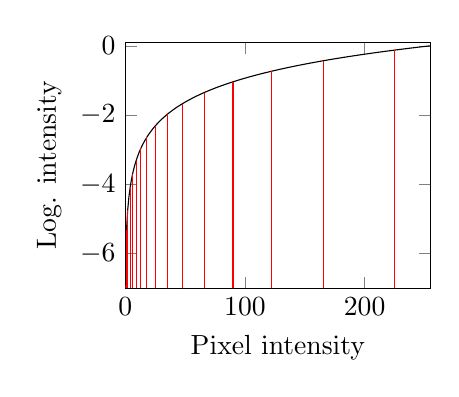
\begin{tikzpicture}
    \begin{axis}[width=.45\linewidth, xmin=0, xmax=255, ymin=-7, ymax=0.1, xlabel={Pixel intensity}, ylabel={Log. intensity}, legend style={nodes={scale=0.7, transform shape}}, legend pos=north west, samples=255]
      \addplot[domain=0:255] {ln(x/255 + 0.001)};
      \draw[red] (0, -7) -- (0, -6.90775527898214);
      \draw[red] (1, -7) -- (1, -5.31412797257468);
      \draw[red] (2, -7) -- (2, -4.72811357220378);
      \draw[red] (4, -7) -- (4, -4.09316878313309);
      \draw[red] (6, -7) -- (6, -3.70788240123955);
      \draw[red] (9, -7) -- (9, -3.31609959913297);
      \draw[red] (13, -7) -- (13, -2.95688870541744);
      \draw[red] (18, -7) -- (18, -2.636824530050834);
      \draw[red] (25, -7) -- (25, -2.31223938923841);
      \draw[red] (35, -7) -- (35, -1.97865618198742);
      \draw[red] (48, -7) -- (48, -1.66476409579933);
      \draw[red] (66, -7) -- (66, -1.34775261144183);
      \draw[red] (90, -7) -- (90, -1.038624547818);
      \draw[red] (122, -7) -- (122, -0.735154517844318);
      \draw[red] (166, -7) -- (166, -0.427740790886742);
      \draw[red] (225, -7) -- (225, -0.124030451358072);
    \end{axis}
  \end{tikzpicture}
  \hfill
  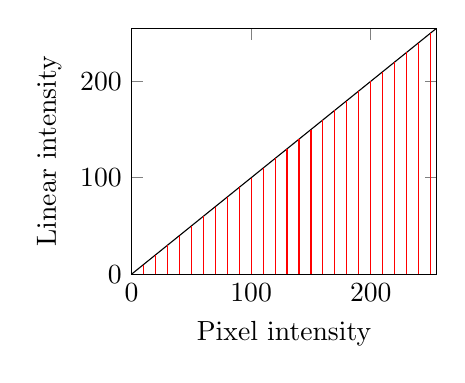
\begin{tikzpicture}
    \begin{axis}[width=.45\linewidth, xmin=0, xmax=255, ymin=0, ymax=255, xlabel={Pixel intensity}, ylabel={Linear intensity}, legend style={nodes={scale=0.7, transform shape}}, legend pos=north west, samples=255]
      \addplot[domain=0:255] {x};
      \pgfplotsinvokeforeach{0,10,...,255} {
        \draw[red] (#1, 0) -- (#1, #1);
      }
    \end{axis}
  \end{tikzpicture}
  \caption{Comparison of the triggering of events when the logarithmic and the linear scales are used. The logarithmic intensity in CARLA is computed as \(\ln(I/255 + 0.001)\), where \(I\) is the pixel intensity. Each red vertical line denotes the triggering of an event, with thresholds set to 0.3 for the logarithmic scale, and 10 for the linear scale.}\label{fig:aled:carla_evts_logs_vs_linear_plots}
  
  \vspace{10mm}

  \begin{subfigure}{0.525\linewidth}
    \centering
    \includegraphics[width=\textwidth]{mainmatter/figures/4_depth_conv/carla_evts_logs_vs_linear/rgb.png}
    \caption{Generated RGB image}
  \end{subfigure}
  \begin{subfigure}{0.475\linewidth}
    \centering
    \includegraphics[width=\textwidth]{mainmatter/figures/4_depth_conv/carla_evts_logs_vs_linear/evts_log_lightgray_fixed.png}
    \caption{Events generated with log.\ scale}
  \end{subfigure}
  \begin{subfigure}{0.475\linewidth}
    \centering
    \includegraphics[width=\textwidth]{mainmatter/figures/4_depth_conv/carla_evts_logs_vs_linear/evts_linear_lightgray_fixed.png}
    \caption{Events generated with linear scale}
  \end{subfigure}
  \caption{Visual comparison of the triggering of events when the logarithmic and the linear scales are used for a urban scene in CARLA. With the logarithmic scale, notice how the dark building on the right generates a high amount of events compared to the other buildings, and how details such as road markings or shadows are mostly lost. In comparison, with the linear scale, notice how the events are better distributed in the image, looking more like what an actual event camera would produce.}\label{fig:aled:carla_evts_logs_vs_linear_imgs}
\end{figure}

We also configured the event camera in CARLA to use a linear intensity scale rather than the default logarithmic one, making the events produced by the simulator more realistic. We argue here that the logarithmic scale amplifies too much the creation of events in the dark areas of the image, as a very slight change in the intensity results in a large logarithmic intensity change, thus triggering an event. On the contrary, in the clearer areas, little to no events are produced, as a large intensity change is necessary to generate a logarithmic difference sufficient to trigger an event. An illustration of this phenomenon is given in \cref{fig:aled:carla_evts_logs_vs_linear_plots,fig:aled:carla_evts_logs_vs_linear_imgs}.

LiDAR data also had to be corrected, due to incorrect values being reported by CARLA in specific cases\footnote{Some objects in CARLA lack the necessary collisions for them to be seen by the LiDAR sensor. For more details, see the following issue, which is still not fully solved despite having been closed: \url{https://github.com/carla-simulator/carla/issues/5732}}. For that purpose, the depth of all LiDAR points was extracted from the corresponding pixels in the ground truth depth maps, instead of using the values given by the sensor.

Finally, we give in \cref{fig:aled:sled_content} an overview of the data contained in the dataset. In particular, we display here illustrations from two very different recordings: one on \verb|Town01| during daytime, and a second one on \verb|Town07| during nighttime.

\begin{figure}
  \centering
  \setlength\tabcolsep{1pt}
  \begin{tabular}{@{}cccc@{}}
    RGB & Depth Map & Events & LiDAR \\
    \includegraphics[width=0.245\linewidth]{mainmatter/figures/4_depth_conv/sled_content/Town01_04_rgb.png} &
    \includegraphics[width=0.245\linewidth]{mainmatter/figures/4_depth_conv/sled_content/Town01_04_depth.png} &
    \includegraphics[width=0.245\linewidth]{mainmatter/figures/4_depth_conv/sled_content/Town01_04_events_lightgray_fixed.png} &
    \includegraphics[width=0.245\linewidth]{mainmatter/figures/4_depth_conv/sled_content/Town01_04_lidar_lightgray_fixed.png} \\
    \includegraphics[width=0.245\linewidth]{mainmatter/figures/4_depth_conv/sled_content/Town07_00_rgb.png} &
    \includegraphics[width=0.245\linewidth]{mainmatter/figures/4_depth_conv/sled_content/Town07_00_depth.png} &
    \includegraphics[width=0.245\linewidth]{mainmatter/figures/4_depth_conv/sled_content/Town07_00_events_lightgray_fixed.png} &
    \includegraphics[width=0.245\linewidth]{mainmatter/figures/4_depth_conv/sled_content/Town07_00_lidar_lightgray_fixed.png}
  \end{tabular}
  \includegraphics[width=0.35\linewidth]{mainmatter/figures/4_depth_conv/sled_content/scale.png} \\
  \begin{tikzpicture}
    \node[] (black) {0m};
    \node[right=1.1cm of black] (pink) {100m};
    \node[right=0.8cm of pink] (yellow) {200m};
  \end{tikzpicture}
  \cprotect\caption{Example data from the \verb|Town01_04| (top) and \verb|Town07_00| (bottom) sequences from our \acrshort{sled} dataset. A color scale is also provided for a better comprehension of the depth values.}\label{fig:aled:sled_content}
\end{figure}


\section{Evaluation}\label{sec:aled:eval}
We split our evaluation to cover the various use cases of our method: estimating dense depth maps, associating two depths to each event, and computing depth change maps.

\subsection{Training Details}
For training on all datasets, we use the Adam optimizer~\cite{Kingma2015AdamAM} with a batch size of 4. When training from scratch on the \acrshort{sled} and the MVSEC datasets, 50 epochs are used, with a fixed learning rate of \(10^{-4}\). When finetuning on the MVSEC dataset, 5 epochs are used, with a learning rate of \(10^{-5}\).

To augment the input data for the \acrshort{sled} dataset, we randomly crop it to \(608 \times 608\), and apply random horizontal flipping. For the MVSEC dataset, we crop it to \(256 \times 256\) (due to the lower resolution), and also apply random horizontal flipping.

\subsection{Evaluation of the Dense Depths}

\subsubsection{On the \acrshort{sled} Dataset}
We begin by training \acrshort{aled} solely on the \acrshort{sled} dataset, and denote it ALED\textsubscript{SL}. Numerical results of ALED\textsubscript{SL} on the testing set of the \acrshort{sled} dataset are presented in the ``Dense depths errors'' column of \cref{tab:aled:results_sled}. Evaluations are conducted on \verb|Town01| and \verb|Town03| maps, which contain challenging environments with many unique features (bridges, tunnels, \dots) that are not present in the training maps. For the max range of 200 meters, ALED\textsubscript{SL} estimates depth maps with an average absolute error slightly over 4.5 meters for \verb|Town01|, and around 5 meters for \verb|Town03|. The respective absolute relative error is around 19\% for \verb|Town01|, and around 22\% for \verb|Town03|.

\begin{table}[ht]
  \centering
  \setlength\tabcolsep{6pt}
  \resizebox{\linewidth}{!}{
    \begin{tabular}{@{}l c cccc cccc cc@{}}
      \toprule
      & \multirow{3}[3]{*}{\textbf{Cutoff}} & \multicolumn{4}{c}{\textbf{Dense depths errors}} & \multicolumn{4}{c}{\textbf{Sparse depths errors}} & \multicolumn{2}{c}{\textbf{Depth change map errors}} \\
      \cmidrule(lr){3-6} \cmidrule(lr){7-10} \cmidrule(lr){11-12}
      & & \multicolumn{2}{c}{On \(D_\text{bf}\)} & \multicolumn{2}{c}{On \(D_\text{af}\)} & \multicolumn{2}{c}{On \(D_\text{bf}\)} & \multicolumn{2}{c}{On \(D_\text{af}\)} & \multirow{2}[1]{*}{Mean (m)} & Correctly classified events (\%) \\
      \cmidrule(lr){3-4} \cmidrule(lr){5-6} \cmidrule(lr){7-8} \cmidrule(lr){9-10}
      & & Mean (m) & AbsRel & Mean (m) & AbsRel & \acrshort{nn} (m) & ALED\textsubscript{SL} (m) & \acrshort{nn} (m) & ALED\textsubscript{SL} (m) & & (with a threshold of \rpm{}1m) \\
      \midrule
      \multirow{5}{*}{\Verb|Town01|} & 10m & 1.24 & 0.201 & 1.37 & 0.236 & 1.32 & 1.46 & 2.24 & 1.79 & 2.11 & 90.27 \\
      & 20m & 2.08 & 0.231 & 2.27 & 0.255 & 1.51 & 1.84 & 2.53 & 2.15 & 3.18 & 85.07 \\
      & 30m & 2.72 & 0.238 & 2.92 & 0.260 & 1.71 & 2.37 & 2.83 & 2.67 & 3.88 & 81.68 \\
      & 100m & 4.25 & 0.240 & 4.51 & 0.261 & 2.40 & 3.48 & 3.91 & 3.95 & 5.12 & 77.48 \\
      & 200m & 4.53 & 0.172 & 4.81 & 0.187 & 7.86 & 5.44 & 9.76 & 6.23 & 7.36 & 75.54 \\
      \midrule
      \multirow{5}{*}{\Verb|Town03|} & 10m & 2.00 & 0.289 & 2.09 & 0.301 & 0.47 & 0.56 & 0.67 & 0.66 & 1.14 & 93.70 \\
      & 20m & 2.85 & 0.299 & 2.97 & 0.311 & 0.64 & 0.75 & 1.12 & 0.87 & 2.54 & 87.16 \\
      & 30m & 3.33 & 0.291 & 3.45 & 0.302 & 0.92 & 1.11 & 1.61 & 1.26 & 3.23 & 83.71 \\
      & 100m & 4.60 & 0.274 & 4.77 & 0.284 & 1.88 & 2.55 & 3.17 & 2.88 & 4.47 & 78.50 \\
      & 200m & 4.86 & 0.215 & 5.03 & 0.223 & 4.43 & 3.60 & 5.93 & 4.10 & 6.20 & 77.23 \\
      \bottomrule
    \end{tabular}
  }
  \caption{Errors on the testing set of the \acrshort{sled} dataset for various cutoff depth distances. From left to right: average absolute and relative depth errors on both the ``before'' \(D_\text{bf}\) and ``after'' \(D_\text{af}\) depth maps; average absolute depth errors when associating a depth to each event; average absolute depth difference errors and percentage of correctly classified events based on this depth difference.}\label{tab:aled:results_sled}
\end{table}

\begin{figure}
  \centering\setlength\tabcolsep{1pt}
  \renewcommand{\arraystretch}{0.5}
  \begin{tabular}{@{}ccc@{}}
    \raisebox{1.9cm}[0pt][0pt]{\rotatebox[origin=c]{90}{Events}} &
    \includegraphics[width=0.475\linewidth]{mainmatter/figures/4_depth_conv/sled_dense_cmp/evts001662_lightgray_fixed.png} &
    \includegraphics[width=0.475\linewidth]{mainmatter/figures/4_depth_conv/sled_dense_cmp/evts007812_lightgray_fixed.png} \\
    \raisebox{1.9cm}[0pt][0pt]{\rotatebox[origin=c]{90}{LiDAR}} &
    \includegraphics[width=0.475\linewidth]{mainmatter/figures/4_depth_conv/sled_dense_cmp/lidar001662_lightgray_fixed.png} &
    \includegraphics[width=0.475\linewidth]{mainmatter/figures/4_depth_conv/sled_dense_cmp/lidar007812_lightgray_fixed.png} \\
    \raisebox{1.9cm}[0pt][0pt]{\rotatebox[origin=c]{90}{Predicted \(D_\text{bf}\)}} &
    \includegraphics[width=0.475\linewidth]{mainmatter/figures/4_depth_conv/sled_dense_cmp/prev001662.png} &
    \includegraphics[width=0.475\linewidth]{mainmatter/figures/4_depth_conv/sled_dense_cmp/prev007812.png} \\
    \raisebox{1.9cm}[0pt][0pt]{\rotatebox[origin=c]{90}{Predicted \(D_\text{af}\)}} &
    \includegraphics[width=0.475\linewidth]{mainmatter/figures/4_depth_conv/sled_dense_cmp/curr001662.png} &
    \includegraphics[width=0.475\linewidth]{mainmatter/figures/4_depth_conv/sled_dense_cmp/curr007812.png} \\
    \raisebox{1.9cm}[0pt][0pt]{\rotatebox[origin=c]{90}{Ground truth (\(D_\text{bf}\))}} &
    \includegraphics[width=0.475\linewidth]{mainmatter/figures/4_depth_conv/sled_dense_cmp/gtprev001662.png} &
    \includegraphics[width=0.475\linewidth]{mainmatter/figures/4_depth_conv/sled_dense_cmp/gtprev007812.png} \\
    & \multicolumn{2}{c}{\includegraphics[width=0.475\linewidth]{mainmatter/figures/4_depth_conv/sled_content/scale.png}} \\
    & \multicolumn{2}{c}{
      \begin{tikzpicture}
        \node[] (black) {0m};
        \node[right=2.2cm of black] (pink) {100m};
        \node[right=1.6cm of pink] (yellow) {200m};
      \end{tikzpicture}
    }
  \end{tabular}
  \cprotect\caption{Two qualitative results on our synthetic \acrshort{sled} dataset, on \verb|Town01| (left) and \verb|Town03| (right). From top to bottom: events, LiDAR, predicted depth maps (\(D_\text{bf}\) and \(D_\text{af}\)), ground truth (\(D_\text{bf}\) only, \(D_\text{af}\) being visually similar), color scale.}\label{fig:aled:sled_dense_cmp}
\end{figure}

A first element that can explain these errors is that the LiDAR has a small vertical coverage of the image: close ground objects or the top of close buildings are not reached by the LiDAR, meaning that accurate depth estimations for these objects are complex to achieve. In opposition, sky pixels (for which ALED\textsubscript{SL} produces good results) are only accounted for at the full 200m cutoff. These observations can be correlated to the larger relative errors observed for close cutoff distances than for the full 200m cutoff. It can also be observed that errors on the ``after'' depth maps are slightly higher. This is to be expected, as the network has to make use of the events to estimate the movement and propagate the depths accordingly. If the reader is interested, results for each sequence of the testing set are given in \cref{sec:appendix:aled:sled_full}.

Qualitative results are given in \cref{fig:aled:sled_dense_cmp}. They showcase the ability of the network to estimate accurate depths for the whole image, by using events as a guide for the areas the LiDAR sensor can not reach. This is particularly visible for the trees and the light pole for the left column, or the ceiling of the tunnel for the right column. If the reader is interested, more visual results are given in \cref{sec:appendix:aled:sled_cmp_additional} and in the videos accessible through the link of the project page given at the very beginning of this chapter (\cpageref{sec:aled}).

\subsubsection{On the MVSEC Dataset}

In order to be able to compare our results with the other approaches in the literature, we also train and evaluate \acrshort{aled} on the MVSEC dataset~\cite{Zhu2018TheMS}. We conduct our evaluation under three different sets of weights from different training setups described below:
\begin{itemize}
  \item ALED\textsubscript{SL}: we reuse the weights trained on proposed \acrshort{sled} dataset;
  \item ALED\textsubscript{MV}: we train a new set of weights on the MVSEC dataset;
  \item ALED\textsubscript{SL\(\rightarrow\)MV}: we reuse the weights trained on \acrshort{sled} and finetune them on the MVSEC dataset.
\end{itemize}

\begin{table}[ht]
  \setlength\tabcolsep{6pt}
  \resizebox{\linewidth}{!}{
    \begin{tabular}{@{}l c c cc cccc@{}}
      \toprule
      & \multirow{2}{*}{\textbf{Cutoff}} & \textbf{Events (stereo)} & \multicolumn{2}{c}{\textbf{Events \& Frames}} & \multicolumn{4}{c}{\textbf{Events \& LiDAR}} \\
      \cmidrule(lr){3-3} \cmidrule(lr){4-5} \cmidrule(lr){6-9}
      & & StereoSpike~\cite{Ranon2021StereoSpikeDL} & RAMNet~\cite{Gehrig2021CombiningEA} & EvT\textsuperscript{+}~\cite{Sabater2022EventTA+} & Cui \textit{et al.}~\cite{Cui2022DenseDE} & \textbf{ALED\textsubscript{SL}} & \textbf{ALED\textsubscript{MV}} & \textbf{ALED\textsubscript{SL\(\rightarrow\)MV}} \\
      \midrule
      \multirow{5}{*}{\Verb|outdoor_day_1|} & 10m & \underline{0.79} & 1.39 & 1.24 & 1.24 & 1.54 & 0.91 & \textbf{0.50} \\
      & 20m & 1.47 & 2.17 & 1.91 & 1.28 & 2.55 & \underline{1.22} & \textbf{0.80} \\
      & 30m & 1.92 & 2.76 & 2.36 & 4.87 & 3.18 & \underline{1.43} & \textbf{1.02} \\
      & 50m & - & - & - & - & 3.79 & \underline{1.67} & \textbf{1.31} \\
      & 100m & 3.17 & - & - & - & 4.08 & \underline{1.96} & \textbf{1.60} \\
      \midrule
      \multirow{5}{*}{\Verb|outdoor_night_1|} & 10m & \textbf{1.38} & 2.50 & \underline{1.45} & 2.26 & 2.24 & 1.75 & 1.52 \\
      & 20m & 2.26 & 3.19 & \underline{2.10} & 2.19 & 3.32 & \underline{2.10} & \textbf{1.81} \\
      & 30m & 2.97 & 3.82 & 2.88 & 4.50 & 3.82 & \underline{2.25} & \textbf{1.95} \\
      & 50m & - & - & - & - & 4.31 & \underline{2.44} & \textbf{2.20} \\
      & 100m & 4.82 & - & - & - & 4.62 & \underline{2.73} & \textbf{2.54} \\
      \midrule
      \multirow{5}{*}{\Verb|outdoor_night_2|} & 10m & - & 1.21 & 1.48 & 1.88 & 1.94 & \underline{1.19} & \textbf{1.09} \\
      & 20m & - & 2.31 & 2.13 & 2.14 & 2.82 & \underline{1.65} & \textbf{1.49} \\
      & 30m & - & 3.28 & 2.90 & 4.67 & 3.22 & \underline{1.81} & \textbf{1.64} \\
      & 50m & - & - & - & - & 3.58 & \underline{1.95} & \textbf{1.80} \\
      & 100m & - & - & - & - & 3.78 & \underline{2.11} & \textbf{1.97} \\
      \midrule
      \multirow{5}{*}{\Verb|outdoor_night_3|} & 10m & - & 1.01 & 1.38 & 1.78 & 1.76 & \underline{0.85} & \textbf{0.81} \\
      & 20m & - & 2.34 & 2.03 & 1.93 & 2.43 & \underline{1.25} & \textbf{1.16} \\
      & 30m & - & 3.43 & 2.77 & 4.55 & 2.78 & \underline{1.42} & \textbf{1.33} \\
      & 50m & - & - & - & - & 3.12 & \underline{1.57} & \textbf{1.51} \\
      & 100m & - & - & - & - & 3.31 & \underline{1.73} & \textbf{1.66} \\
      \bottomrule
    \end{tabular}
  }
  \caption{Average absolute depth errors (in meters) on the MVSEC dataset for various cutoff depth distances. This evaluation is performed on the ``before'' depth map \(D_\text{bf}\), to be consistent with the methods we compare ourselves to.}\label{tab:aled:results_mvsec}
\end{table}

Numerical results of all three variants are given in \cref{tab:aled:results_mvsec}. Comparing them, it appears clearly that training on synthetic data before finetuning the network on the MVSEC dataset (ALED\textsubscript{SL\(\rightarrow\)MV}) produces the best results. Training from zero on the MVSEC dataset (ALED\textsubscript{MV}) is not as good as the ALED\textsubscript{SL\(\rightarrow\)MV} variant due to the limited data available for training. Finally, training solely on the \acrshort{sled} dataset (ALED\textsubscript{SL}) produces the worst results, due to the large differences in terms of resolution and LiDAR models between the two datasets, and as simulation is not a perfect reproduction of real data.

Our ALED\textsubscript{SL\(\rightarrow\)MV} network greatly outperforms all the other approaches of the state of the art. Most impressive results are obtained with distant cutoff depths, where fewer LiDAR points are available; our network is still able to infer accurate depths, while reference methods show large errors:
\begin{itemize}
  \item compared to the stereo events StereoSpike method of Rançon \textit{et al.}~\cite{Ranon2021StereoSpikeDL}, for the 20m and 30m cutoff distances respectively, we improve the error by 19.9\% and 34.3\% in the worst case, and by 45.6\% and 46.9\% in the best case;
  \item compared to the frames \& events EvT\textsuperscript{+} method of Sabater \textit{et al.}~\cite{Sabater2022EventTA+}, this improvement is of 13.8\% and 32.3\% in the worst case and of 58.1\% and 56.8\% in the best case at maximum;
  \item compared to the LiDAR \& events method of Cui \textit{et al.}~\cite{Cui2022DenseDE}, this improvement is of 17.4\% and 56.7\% in the worst case and of 39.9\% and 79.1\% in the best case.
\end{itemize}

\begin{figure}
  \centering
  \begin{subfigure}{0.31\textwidth}
    \centering
    \includegraphics[width=\textwidth]{mainmatter/figures/4_depth_conv/mvsec_cmp/img.png}
    \caption{Reference image}
  \end{subfigure}
  \hfill
  \begin{subfigure}{0.31\textwidth}
    \centering
    \includegraphics[width=\textwidth]{mainmatter/figures/4_depth_conv/mvsec_cmp/evts_ours_cropped_lightgray_fixed.png}
    \caption{Events input}
  \end{subfigure}
  \hfill
  \begin{subfigure}{0.31\textwidth}
    \centering
    \includegraphics[width=\textwidth]{mainmatter/figures/4_depth_conv/mvsec_cmp/lidar_cropped_lightgray_fixed.png}
    \caption{LiDAR input}
  \end{subfigure}
  \begin{subfigure}{0.31\textwidth}
    \centering
    \includegraphics[width=\textwidth]{mainmatter/figures/4_depth_conv/mvsec_cmp/ours_s_cropped.png}
    \caption{ALED\textsubscript{SL}}
  \end{subfigure}
  \hfill
  \begin{subfigure}{0.31\textwidth}
    \centering
    \includegraphics[width=\textwidth]{mainmatter/figures/4_depth_conv/mvsec_cmp/ours_r_cropped.png}
    \caption{ALED\textsubscript{MV}}\label{subfig:aled:mvsec_cmp:mv}
  \end{subfigure}
  \hfill
  \begin{subfigure}{0.31\textwidth}
    \centering
    \includegraphics[width=\textwidth]{mainmatter/figures/4_depth_conv/mvsec_cmp/ours_sr_cropped.png}
    \caption{ALED\textsubscript{SL\(\rightarrow\)MV}}\label{subfig:aled:mvsec_cmp:sl_mv}
  \end{subfigure}
  \begin{subfigure}{0.31\textwidth}
    \centering
    \includegraphics[width=\textwidth]{mainmatter/figures/4_depth_conv/mvsec_cmp/ramnet_cvt.png}
    \caption{RAMNet~\cite{Gehrig2021CombiningEA}}
  \end{subfigure}
  \hfill
  \begin{subfigure}{0.31\textwidth}
    \centering
    \includegraphics[width=\textwidth]{mainmatter/figures/4_depth_conv/mvsec_cmp/gt_ours_cropped_lightgray_fixed.png}
    \caption{Ground truth}
  \end{subfigure}
  \hfill
  \begin{subfigure}{0.31\textwidth}
    \centering
    \vspace{10mm}
    \includegraphics[width=0.8\textwidth]{mainmatter/figures/4_depth_conv/sled_content/scale.png}
    \begin{tikzpicture}
      \node[] (black) {0m};
      \node[right=0.6cm of black] (pink) {50m};
      \node[right=0.3cm of pink] (yellow) {100m};
    \end{tikzpicture}
    \vspace{6mm}
    \caption{Scale}
  \end{subfigure}
  \cprotect\caption{Qualitative results on the \verb|outdoor_day_1| sequence from the MVSEC dataset.}\label{fig:aled:mvsec_cmp}
\end{figure}

Qualitative results are presented in \cref{fig:aled:mvsec_cmp}. All three \acrshort{aled} variants produce results which are visually close to the ground truth for ground objects. Since the MVSEC dataset lacks ground truth depth for the sky, and since the rare elements to have a ground truth for this part of the image are close buildings, close trees, or power lines, the network cannot learn to derive correct depth estimations for the corresponding pixels, leading to the purple blobs in the upper parts of \cref{subfig:aled:mvsec_cmp:mv,subfig:aled:mvsec_cmp:sl_mv}. Only the ALED\textsubscript{SL} variant is able to predict accurate values for sky areas (as our \acrshort{sled} dataset contains valid ground truth depths for all pixels), but has more difficulties for ground objects due to the lack of finetuning. Between the ALED\textsubscript{MV} and ALED\textsubscript{SL\(\rightarrow\)MV} variants, improvement can still be seen, for instance for the edges of the objects of \cref{subfig:aled:mvsec_cmp:mv,subfig:aled:mvsec_cmp:sl_mv}, which are less uneven for the ALED\textsubscript{SL\(\rightarrow\)MV} variant. Finally, when comparing our results to RAMNet, we can clearly observe that our method provides in all cases more accurate depth maps, where object boundaries are more prominent, and where estimated depths are closer to the ground truth. This observation further demonstrates that the use of a LiDAR input --- even if very sparse --- is of great help for obtaining accurate dense depth maps.

If the reader is interested, qualitative results for each of the sequences of the MVSEC dataset are given in \cref{sec:appendix:aled:mvsec_cmp_additional}. Full results are also available in video format through the link of the project page given at the very beginning of this chapter (\cpageref{sec:aled}).

\subsection{Evaluation of the Sparse Depths}\label{sec:aled:eval:sparse}
As stated in \cref{sec:aled:intro,sec:aled:two_depths_per_event}, our goal is not only to estimate dense depth maps, but also to associate two depths to each event, allowing for their 3D reprojection and depth difference analysis. Evaluation of the depth association to each event on proposed \acrshort{sled} dataset is given in the ``Sparse depths errors'' column of \cref{tab:aled:results_sled}.

The sparse event-LiDAR fusion literature is limited to the method of Li \textit{et al.}~\cite{Li2021Enhancing3L}. However, their approach only considers one depth per event, and is intended for a \acrfull{rsu} application (i.e., their event camera is fixed and evaluation is conducted on a specific dataset). Therefore, we decided to compare ourselves to a more naive (and faster) baseline: the \acrfull{nn} approach, where each event is given the depth of its closest LiDAR point. As the \acrlong{nn} approach can not infer correct depths for events which are too far from a LiDAR scan, and so as to provide a fair comparison, we only consider the events between the bottom and top LiDAR scans.

As displayed in \cref{tab:aled:results_sled}, in the ``before'' \(D_\text{bf}\) case, depending on the map and the cutoff distance, best results are shared between the \acrshort{nn} approach and our ALED\textsubscript{SL} network. These results can be explained by the fact that our network is more likely to commit large errors for events at the boundary of close objects, as it might estimate that they should be given the depth of the more distant background. On the contrary, the \acrshort{nn} approach will always attribute the depth of the closest LiDAR point, and will therefore commit more frequent but smaller errors. In the ``after'' \(D_\text{af}\) case, despite this potential source of error, our network ALED\textsubscript{SL} nearly always obtains the best results, as it has correctly learned the temporal propagation of the depths, a task which cannot be completed natively with the \acrshort{nn} approach. We also remind here that these results are given for the parts of the image where LiDAR data is available: the \acrshort{nn} method would not be able to derive correct estimations for the other parts of the image. If the reader is interested, numerical results for each sequence of the testing set are given in \cref{sec:appendix:aled:sled_full}.

\subsection{Evaluation of the Depth Change Maps}

\begin{figure}
  \centering
  \setlength\tabcolsep{1pt}
  \begin{tabular}{@{}cc@{}}
    Predicted depth change map & Ground truth \\
    \includegraphics[width=0.49\linewidth]{mainmatter/figures/4_depth_conv/sled_diff_cmp/pdiff001662.png} &
    \includegraphics[width=0.49\linewidth]{mainmatter/figures/4_depth_conv/sled_diff_cmp/gtdiff001662.png} \\
    \includegraphics[width=0.49\linewidth]{mainmatter/figures/4_depth_conv/sled_diff_cmp/pdiff007812.png} &
    \includegraphics[width=0.49\linewidth]{mainmatter/figures/4_depth_conv/sled_diff_cmp/gtdiff007812.png}
  \end{tabular}
  \begin{tikzpicture}
    \definecolor{colorblack}{HTML}{000004}
    \definecolor{coloryellow}{HTML}{FCFFA4}
    \definecolor{colorpink}{HTML}{BC3754}
    \node[draw, minimum width=0.25cm, minimum height=0.25cm, fill=colorblack] (black) {};
    \node[draw, minimum width=0.25cm, minimum height=0.25cm, fill=colorpink, below=0.3cm of black] (pink) {};
    \node[draw, minimum width=0.25cm, minimum height=0.25cm, fill=coloryellow, below=0.3cm of pink] (yellow) {};
    \node[right=0.1cm of black] (black_l) {\(d_\text{af} - d_\text{bf} < -1\text{m}\)};
    \node[right=0.1cm of pink] (pink_l) {\(d_\text{af} - d_\text{bf} \in [-1\text{m}, +1\text{m}]\)};
    \node[right=0.1cm of yellow] (yellow_l) {\(d_\text{af} - d_\text{bf} > +1\text{m}\)};
  \end{tikzpicture}
  \cprotect\caption{Thresholded depth change maps from the \verb|Town_01| and \verb|Town_03| sequences of the \acrshort{sled} dataset, using the events as a mask.}\label{fig:aled:sled_diff_cmp}
\end{figure}

We finally estimate the quality of our ``two depths per event'' approach through the depth change map, as presented in \cref{sec:aled:two_depths_per_event}. We perform two evaluations on our \acrshort{sled} dataset:
\begin{enumerate*}[label=\textbf{(\arabic*)}]
  \item the average error on the depth change map \(D_\text{af}-D_\text{bf}\) compared to the true depth changes, and
  \item the percentage of correctly classified events when using a difference threshold of 1m on the depth change map.
\end{enumerate*}
Results of these evaluations are given in the ``Depth change map errors'' column of \cref{tab:aled:results_sled}. If the reader is interested, numerical results for each sequence of the testing set are given in \cref{sec:appendix:aled:sled_full}.

We can observe here that, despite a significant absolute error on the depth change maps, events can still be classified correctly, with a rate of success over 75\% on \verb|Town01|, and over 77\% on \verb|Town03|. We remind here that the ALED network is not trained on these depth change map and classification tasks. As such, we believe that, while even more accurate individual depth maps could improve both the depth change map and classification errors, further improvements could be brought by designing a network specifically dedicated to these tasks.

We show in \cref{fig:aled:sled_diff_cmp} qualitative results for the thresholded depth change maps, for the same sequences as in \cref{fig:aled:sled_dense_cmp}. These results visually corroborate the overall accurate classification of the events observed during the numerical analysis. Some errors can still be seen, especially for the lower parts of the objects: as they are closer to the ground, the depth difference is less significant, and errors on the depth change map become therefore more critical. More qualitative results are given in \cref{sec:appendix:aled:sled_diff_cmp_add}.


\section{Conclusion and Discussions}\label{sec:aled:conclusion}
Throughout this chapter, a novel learning-based approach for estimating dense depth maps from asynchronous LiDAR and event-based data has been proposed. A novel ``two depths per event'' notion has also been proposed, to solve the issue of events possibly representing a change of depth. A synthetic multimodal dataset has also been recorded, to train and evaluate our method. Multiple evaluations on our synthetic and a real driving datasets have been performed to show the relevance of our contributions. In particular, on the MVSEC dataset, an improvement of up to 79.1\% compared to the current LiDAR-and-events state of the art has been achieved, on complex daytime and nighttime recordings.

In hindsight, further improvements could be brought to the method.
\begin{enumerate*}[label=\textbf{(\arabic*)}]
  \item Making the network predict directly sparse depths for each event could potentially provide better results for the depth to event inference. This could be achieved by using sparse convolutional networks~\cite{Messikommer2020EventbasedAS} for instance, and could be subject to future work.
  \item The use of the Event Volume with a fixed time window as the input representation for the events in our network could also be revised, as it can become ill-suited under large motions. A solution could be to use an alternative representation, such as TORE Volumes~\cite{Baldwin2021TimeOrderedRE}, or to use adaptive accumulation times using methods such as the one proposed by Liu and Delbrück~\cite{Liu2018AdaptiveTB}.
  \item The \acrshort{sled} dataset was recorded so that the ego-vehicle would not get stuck in traffic or in front of traffic lights, to avoid having fully static sequences (as a reminder, sequences last 10 seconds in \acrshort{sled}), because the dense depth estimation would be impossible for these sequences due to a lack of events. However, this means that the ego-vehicle almost never stops across the whole dataset, which is also an issue. An update to \acrshort{sled} could therefore be published in the future, for ensuring that the vehicle makes short stops in some sequences, for more diversity.
  \item Finally, the recording of a real dataset with a high-definition event camera could also be considered, to complete the possibilities offered by the low-resolution MVSEC dataset.
\end{enumerate*}

One of the highlights of this work is how visually impressive the results are, especially given the sparsity of the input data to the network (as shown for instance in \cref{fig:aled:sled_dense_cmp}). In the case of our \acrshort{sled} dataset, the segmentation between the sky and other objects is also an important highlight, even in the case of \cref{fig:appendix:aled:sled_cmp_additional_good_2} where a suspended railway is above the vehicle. Our network also displays good results on the night sequences of the MVSEC dataset, meaning that it is able to perform well even in the presence of noisy events. Yet, looking back at \cref{tab:aled:results_sled,tab:aled:results_mvsec}, our method seems to have more difficulties for short ranges, where the errors are relatively high. If we consider an application to intelligent robotics, this becomes an important issue: the precision of the depth of close objects should be favored compared to the more distant ones, as we primarily want to avoid collisions with objects surrounding the robot.

Therefore, to extend this work on depth estimation, we will look in the following chapter into a more refined method, by making use of the Transformer architecture~\cite{Vaswani2017AttentionIA} and especially its concept of self- and cross-attention. Our idea is that attention-based networks provide state-of-the-art results in numerous vision-based applications, and could further improve the fusion of the event and LiDAR modalities.
